\documentclass{article}

\usepackage[italian]{babel}
\usepackage[margin=2cm, footskip=5mm]{geometry}
% questi package non sono necessari in lualatex; ref https://tex.stackexchange.com/a/413046
% \usepackage[utf8]{inputenc}
% \usepackage[T1]{fontenc}
\usepackage{enumitem}
\usepackage{hyperref}
\usepackage{titlesec}
\usepackage{soulutf8}
\usepackage{contour}
\usepackage{float}
\usepackage{graphicx}
\usepackage{fancyhdr}
\usepackage{longtable}
\usepackage[table]{xcolor}
\usepackage{titling}
\usepackage{lastpage}
\usepackage{ifthen}
\usepackage{calc}
\usepackage{minted}
\usepackage{pgfgantt}
\usepackage{subfiles}

\newlength{\imgwidth}

\newcommand\scalegraphics[1]{%
    \settowidth{\imgwidth}{\includegraphics{#1}}%
    \setlength{\imgwidth}{\minof{\imgwidth}{\textwidth}}%
    \includegraphics[width=\imgwidth]{#1}%
}

% XXX definizione dei percorsi in cui cercare immagini
\graphicspath{ {./}
    {./img/}
}

% esempio di utilizzo: \appendToGraphicspath{./img/} (un comando diverso per ogni path da includere)
% N.B.: ci DEVE essere un forward slash alla fine del path, a indicare che è una cartella.
\makeatletter
\newcommand\appendToGraphicspath[1]{%
  \g@addto@macro\Ginput@path{{#1}}%
}
\makeatother

% setup della sottolineatura
\setuldepth{Flat}
\contourlength{0.8pt}

\newcommand{\uline}[1]{%
  \ul{{\phantom{#1}}}%
  \llap{\contour{white}{#1}}%
}

% setup dei link
\hypersetup{
  colorlinks=true, % set true if you want colored links
  linktoc=all,     % set to all if you want both sections and subsections linked
  linkcolor=black, % choose some color if you want links to stand out
}

% setup di header e footer
\pagestyle{fancy}

\fancyhf{}
\fancyhead[L]{\includegraphics[width=1cm]{logo.png}}
\fancyhead[R]{\thetitle}
\fancyfoot[R]{\thepage\ di~\pageref{LastPage}}

\fancypagestyle{nopage}{%
  \fancyfoot{}%
}

\setlength{\headheight}{1.2cm}

% setup forma \paragraph e \subparagraph
\titleformat{\paragraph}[hang]{\normalfont\normalsize\bfseries}{\theparagraph}{1em}{}
\titleformat{\subparagraph}[hang]{\normalfont\normalsize\bfseries}{\thesubparagraph}{1em}{}

% setup profondità indice di default
\setcounter{secnumdepth}{5}
\setcounter{tocdepth}{5}

% shortcut per i placeholder
\newcommand{\plchold}[1]{\textit{\{#1\}}} % chktex 20

% hook per lo script che genera il glossario
\newcommand{\glossario}[1]{\underline{#1}\textsubscript{g}}

% definizione dei comandi \uso e \stato
\makeatletter
\newcommand{\setUso}[1]{%
  \newcommand{\@uso}{#1}%
}
\newcommand{\uso}{\@uso}

\newcommand{\setStato}[1]{%
  \newcommand{\@stato}{#1}%
}
\newcommand{\stato}{\@stato}

\newcommand{\setVersione}[1]{%
  \newcommand{\@versione}{#1}%
}
\newcommand{\versione}{\@versione}

\newcommand{\setResponsabile}[1]{%
  \newcommand{\@responsabile}{#1}%
}
\newcommand{\responsabile}{\@responsabile}

\newcommand{\setRedattori}[1]{%
  \newcommand{\@redattori}{#1}%
}
\newcommand{\redattori}{\@redattori}

\newcommand{\setVerificatori}[1]{%
  \newcommand{\@verificatori}{#1}%
}
\newcommand{\verificatori}{\@verificatori}

\newcommand{\setDescrizione}[1]{%
  \newcommand{\@descrizione}{#1}%
}
\newcommand{\descrizione}{\@descrizione}

\newcommand{\setModifiche}[1]{%
  \newcommand{\@modifiche}{#1}%
}

\newcommand{\modifiche}{\@modifiche}

\makeatother

% setup delle description
\setlist[description,1]{font=$\bullet$\hspace{1.5mm}, labelwidth=* leftmargin=*,labelindent=12.5mm}
\setlist[description,2]{font=$\bullet$\hspace{1.5mm}, leftmargin=*,labelindent=12.5mm}
\appendToGraphicspath{../../commons/img/}

\title{Studio di Fattibilità}

\setVersione{\plchold{versione}}
\setResponsabile{Alessandro Rizzo}
\setRedattori{
  Tobia Apolloni \\ &
  Riccardo Cestaro \\ &
  Alberto Cocco \\ &
  Alberto Gobbo \\ &
  Alessandro Rizzo \\ &
  Fabio Scettro
}
\setVerificatori{
  Riccardo Agatea \\ &
  Luca Ercole
}
\setStato{WIP}
\setUso{Interno}
\setDescrizione{Studio di fattibilità sui capitolati proposti al corso di Ingegneria del Software a.a. 2019--2020}
\setModifiche{%
0.0.3 & Riccardo Agatea & 2019--12--07 & approva il documento \\%
0.0.2 & Riccardo Agatea, Luca Ercole & 2019--12--07 & revisiona il documento\\%
0.0.2 & Alessandro Rizzo & 2019--12--07 & aggiungi riferimenti al glossario \\%
0.0.2 & Fabio Scettro & 2019--12--06 & correggi studio di fattibilità \\%
0.0.2 & Riccardo Agatea & 2019--12--05 & revisiona il documento e segnala gli errori\\%
0.0.2 & Alessandro Rizzo & 2019--12--04 & aggiungi lo studio di fattibilità  di C6 \\%
0.0.2 & Alessandro Rizzo & 2019--12--03 & aggiungi lo studio di fattibilità  di C4 \\%
0.0.2 & Alessandro Rizzo & 2019--12--02 & aggiungi lo studio di fattibilità  di C3 \\%
0.0.2 & Alessandro Rizzo & 2019--12--01 & aggiungi lo studio di fattibilità  di C2 \\%
0.0.2 & Alessandro Rizzo & 2019--11--29 & aggiungi lo studio di fattibilità  di C1 \\%
0.0.2 & Alessandro Rizzo & 2019--11--27 & aggiungi lo studio di fattibilità  di C5 \\%
0.0.2 & Alessandro Rizzo & 2019--11--23 & aggiungi collegamenti per i sottofile \\%
0.0.2 & Luca Ercole & 2019--11--23 & aggiungi redattori e verificatori sui documenti \\%
0.0.2 & Luca Ercole & 2019--11--22 & crea documenti vuoti con template \\%
}

\begin{document}

\thispagestyle{empty}
\pagenumbering{gobble}

\begin{center}

  \includegraphics[width=8.5cm]{\commons/img/logo.png}\\
  {\Large GruppOne - progetto "Stalker"}\\
  \vspace{1.5cm}

  {\Huge \thetitle}
  \vspace{1.5cm}

  \begin{table}[H]
    \centering

    \begin{tabular}{r|l}
      \textbf{Versione}     & \versione              \\
      \textbf{Approvazione} & \responsabile          \\
      \textbf{Redazione}    & \redattori             \\
      \textbf{Verifica}     & \verificatori          \\
      \textbf{Stato}        & \stato                 \\
      \textbf{Uso}          & \uso                   \\
      \textbf{Destinato a}  & Imola Informatica      \\
                            & GruppOne               \\
                            & Prof. Tullio Vardanega \\
                            & Prof. Riccardo Cardin  \\
    \end{tabular}
  \end{table}

  \vspace{3cm}
  \textbf{Descrizione}\\
  \descrizione\\
  \vfill
  \verb|gruppone.swe@gmail.com|
\end{center}

\newpage
\thispagestyle{nopage}

\section*{Registro delle modifiche}
\label{sec:registro_delle_modifiche}

\begin{table}[H]
  \label{tab:registro_delle_modifiche}

  \centering
  \rowcolors{2}{lightgray}{white!80!lightgray!100}

  \begin{longtable}[c]{c c c c l}
    \rowcolor{darkgray!90!}\color{white}{\textbf{Versione}} & \color{white}{\textbf{Data}} & \color{white}{\textbf{Nominativo}} & \color{white}{\textbf{Ruolo}} & \color{white}{\textbf{Descrizione}} \\\endhead
    \modifiche
  \end{longtable}
\end{table}

% section registro_delle_modifiche (end)
\newpage

\thispagestyle{nopage}
\pagenumbering{roman}
\tableofcontents

\newpage

\pagenumbering{arabic}


\section{Capitolato C5 --- Stalker}
\subfile{components/fattibilita-c5.tex}

\newpage
\section{Capitolato C1 --- Autonomous highlights platform}
\subfile{components/fattibilita-c1.tex}

\newpage
\section{Capitolato C2 --- Etherless}
\subfile{components/fattibilita-c2.tex}

\newpage
\section{Capitolato C3 --- NaturalAPI}
\subfile{components/fattibilita-c3.tex}

\newpage
\section{Capitolato C4 --- Predire in Grafana}
\subfile{components/fattibilita-c4.tex}

\newpage
\section{Capitolato C6 --- ThiReMa}
\subfile{components/fattibilita-c6.tex}

\end{document}
